\documentclass[titlepage, a4paper]{article}
\usepackage[swedish]{babel}
\usepackage[utf8]{inputenc}
\usepackage{color}
\usepackage{graphicx}
\usepackage{etoolbox}
\usepackage{stringenc}
\usepackage{pdfescape}

% Sidformat
\usepackage{a4wide}

% Fixa Appendix-titlar
\usepackage[titletoc,title]{appendix}

% Bättre tabeller
\usepackage{tabularx}

% Bättre bildtexter
\usepackage[margin=10pt,font=small,labelfont=bf,labelsep=endash]{caption}

% Enkelt kommando som låter mig attgöra-markera text
\newcommand{\todo}[1] {\textbf{\textcolor{red}{#1}}}

% Nytt \paragraph låter oss ha onumrerade bitar
\makeatletter
\renewcommand\paragraph{\@startsection{paragraph}{4}{\z@}%
{-3.25ex\@plus -1ex \@minus -.2ex}%
{1.5ex \@plus .2ex}%
{\normalfont\normalsize\bfseries}}
\makeatother

\providecommand{\LIPSlogga}{../mall/logga2.png}
\providecommand{\LIPSdatum}{\today}

%% Headers och Footers
\usepackage{fancyhdr}
\pagestyle{fancy}
\lhead{\includegraphics[scale=0.4]{\LIPSlogga}}
\rhead{\ifdef{\LIPSutfardare}{Utfärdat av \LIPSutfardare \\\LIPSdatum}\LIPSdatum}
\lfoot{\LIPSkursnamn \\ \LIPSdokumenttyp}
\cfoot{\thepage}
\rfoot{ \LIPSprojektnamn}

%% Titelsida
\newcommand{\LIPSTitelsida}{%
{\ }\vspace{45mm}
\begin{center}
  \textbf{\Huge \LIPSdokument}
\end{center}
\begin{center}
{\Huge \LIPSprojektnamn}
\end{center}
\begin{center}
  {\Large Redaktör: \LIPSredaktor}
\end{center}
\begin{center}
  {\Large \textbf{Version \LIPSversion}}
\end{center}
\vfill
\begin{center}
  {\large Status}\\[1.5ex]
  \begin{tabular}{|*{3}{p{40mm}|}}
    \hline
    Granskad & \LIPSgranskare & \LIPSgranskatdatum \\
    \hline
    Godkänd & \LIPSgodkannare & \LIPSgodkantdatum \\
    \hline
  \end{tabular}
\end{center}
\newpage
}

% Projektidentitet
\newenvironment{LIPSprojektidentitet}{%
{\ }\vspace{45mm}
\begin{center}
  {\Large PROJEKTIDENTITET}\\[0.5ex]
  {\small
  \LIPSartaltermin,\\
  Linköpings Tekniska Högskola, IDA
  }
\end{center}
\begin{center}
  {\normalsize Gruppdeltagare}\\
  \begin{tabular}{|l|l|p{25mm}|l|}
    \hline
    \textbf{Namn} & \textbf{Ansvar} & \textbf{Telefon} & \textbf{E-post} \\
    \hline
}%
{%
    \hline
  \end{tabular}
\end{center}
\begin{center}
  {\small
    \ifdef{\LIPSgruppadress}{\textbf{E-postlista för hela gruppen}: \LIPSgruppadress\\}{}
    \ifdef{\LIPSgrupphemsida}{\textbf{Hemsida}: \LIPSgrupphemsida\\[1ex]}{}
    \ifdef{\LIPSkund}{\textbf{Kund}: \LIPSkund\\}{}
    \ifdef{\LIPSkundkontakt}{\textbf{Kontaktperson hos kund}: \LIPSkundkontakt\\}{}
    \ifdef{\LIPSkursansvarig}{\textbf{Kursansvarig}: \LIPSkursansvarig\\}{}
    \ifdef{\LIPShandledare}{\textbf{Handledare}: \LIPShandledare\\}{}
  }
\end{center}
\newpage
}
\newcommand{\LIPSgruppmedlem}[4]{\hline {#1} & {#2} & {#3} & {#4} \\}

%% Dokumenthistorik
\newenvironment{LIPSdokumenthistorik}{%
\begin{center}
  Dokumenthistorik\\[1ex]
  %\begin{small}
    \begin{tabular}{|l|l|p{60mm}|l|l|}
      \hline
      \textbf{Version} & \textbf{Datum} & \textbf{Utförda förändringar} & \textbf{Utförda av} & \textbf{Granskad} \\
      }%
    {%
			\hline
    \end{tabular}
  %\end{small}
\end{center}
}

\newcommand{\LIPSversionsinfo}[5]{\hline {#1} & {#2} & {#3} & {#4} & {#5} \\}

% Kravlistor
\newenvironment{LIPSkravlista}{
	\center
		\tabularx{\textwidth}{| p{1.2cm} | p{1.9cm} | X | c |}
			\hline
			\textbf{Krav} & \textbf{Förändring} & \textbf{Beskrivning} & \textbf{Prioritet} \\\hline
}
{
		\endtabularx
	\endcenter
}

\newcounter{LIPSkravnummer}
\addtocounter{LIPSkravnummer}{1}
\newcommand{\LIPSkrav}[4][Krav \arabic{LIPSkravnummer}]{{#1} & {#2} & {#3} & {#4} \stepcounter{LIPSkravnummer}\\\hline}


% Leveranskravlistor
\newenvironment{LIPSleveranskravlista}{
	\center
		\tabularx{\textwidth}{| p{1.2cm} | p{1.9cm} | X | X |}
			\hline
			\textbf{Krav} & \textbf{Förändring} & \textbf{Beskrivning} & \textbf{Deadline}\\\hline
}
{
		\endtabularx
	\endcenter
}

\newcounter{LIPSleveranskravnummer}
\addtocounter{LIPSleveranskravnummer}{1}
\newcommand{\LIPSleveranskrav}[4][Krav \arabic{LIPSkravnummer}]{{#1} & {#2} & {#3} & {#4} \stepcounter{LIPSkravnummer}\\\hline}


% Milstolps-lista
\newenvironment{LIPSmilstolpar}{
	\center
		\tabularx{\textwidth}{| p{1.2cm} | X | l |}
			\hline
			\textbf{Nr} & \textbf{Beskrivning} & \textbf{Datum} \\\hline
}
{
		\endtabularx
	\endcenter
}

\newcounter{LIPSstolpnummer}
\addtocounter{LIPSstolpnummer}{1}
%\newcommand{\LIPSmilstolpe}[3][Krav \arabic{LIPSstolpnummer}]{{#1} & {#2} & {#3} \stepcounter{LIPSstolpnummer}\\\hline}
\newcommand{\LIPSmilstolpe}[3]{{#1} & {#2} & {#3} \\\hline}

% Aktivitets-lista
\newenvironment{LIPSaktivitetslista}{
	\center
		\tabularx{\textwidth}{| p{0.3cm} | X | c | c | c |}
			\hline
			\textbf{Nr} & \textbf{Beskrivning} & \textbf{Beroende av} & \textbf{Timmar} & \textbf{datum} \\\hline
}
{
		\endtabularx
	\endcenter
}

\newcounter{LIPSaktivitetsnummer}
\addtocounter{LIPSaktivitetsnummer}{1}
% \newcommand{\LIPSaktivitet}[4][\arabic{LIPSstolpnummer}]{{#1} & {#2} & {#3} & {#4} \stepcounter{LIPSstolpnummer}\\\hline}
\newcommand{\LIPSaktivitet}[5]{{#1} & {#2} & {#3} & {#4} & {#5}\\\hline}

% Mall för mötesprotokoll
\newenvironment{projektmote}[2]{
  {\ }\vspace{5mm}

  \centerline{\textbf{\Huge #1}}
  \vspace{2mm}
  \centerline{\LARGE #2}
  \vspace{10mm}

  \begin{itemize}
}
{
  \end{itemize}
}

\newcounter{paragrafnummer}
\addtocounter{paragrafnummer}{1}
\newcommand{\paragraf}[1]{\item{\textsection \arabic{paragrafnummer}. {#1}}\addtocounter{paragrafnummer}{1}}

% Mall för Statusrapport
\newenvironment{statusrapport}{
  \center
    \tabularx{\textwidth}{| p{0.4cm} | X | X | p{14.5mm} | p{13.5mm} | p{16.5mm} | p{16.5mm} |}
    \hline
    \textbf{Nr} & \textbf{Aktivitet} & \textbf{Beroenden} & \textbf{Planerad tid} & \textbf{Nedlagd tid} & \textbf{Planerad klar} & \textbf{Beräknat klart} \\\hline
}
{
    \endtabularx
  \endcenter
}

\newcommand{\aktivitetstatus}[7]{{#1} & {#2} & {#3} & {#4} & {#5} & {#6} & {#7} \\\hline}	% Importera generella layout-strukturer

% Information nödvändig för generella layout-strukturer
\newcommand{\LIPSgrupp}{50}
\newcommand{\LIPSredaktor}{Martin Söderén}
\newcommand{\LIPSversion}{0.1}
\newcommand{\LIPSdokument}{Rapport}
\newcommand{\LIPSdokumenttyp}{Rapport}
\newcommand{\LIPSgranskatdatum}{-}
\newcommand{\LIPSgranskare}{-}
\newcommand{\LIPSgodkannare}{-}
\newcommand{\LIPSgodkantdatum}{-}
\newcommand{\LIPSkursnamn}{TSBK07}
\newcommand{\LIPSprojektnamn}{TMBTRF 3D File Manager}
\newcommand{\LIPSprojektgrupp}{Grupp 50}
\newcommand{\LIPSartaltermin}{VT, 2016}
\newcommand{\LIPSgrupphemsida}{https://github.com/marso329/tsbk07/tree/master/projekt}
\newcommand{\LIPSkund}{LIU}
\newcommand{\LIPSkundkontakt}{Ingemar Ragnemalm}
\newcommand{\LIPSkursansvarig}{Ingemar Ragnemalm}
\newcommand{\LIPShandledare}{Ingemar Ragnemalm}

% Dokument-specifika paket
\usepackage{tabularx}
\usepackage{tikz}	
\usepackage{amsmath}
\usepackage{amsfonts}
\usepackage{float}
\usepackage{hyperref}
\usetikzlibrary{shapes, arrows}

\pagenumbering{roman}

\begin{document}

\LIPSTitelsida

\begin{LIPSprojektidentitet}
	\LIPSgruppmedlem{Martin Söderén}{Senior Software design engineer}{070 816 32 41}{marso329@student.liu.se}
\end{LIPSprojektidentitet}

%\newpage
%\tableofcontents	%Innehållsförteckning

\newpage

\begin{LIPSdokumenthistorik}
\LIPSversionsinfo{0.1}{2016-05-26}{Första utkast}{Martin}{}
\end{LIPSdokumenthistorik}

\newpage
\pagenumbering{arabic}	%Påbörja sidnumrering

\section{Inledning}
Jag har gjort en filhanterar som visualiserar alla filer och mappar i 3D med hjälp av OpenGL. Inspirationen till detta projekt var bland annat FSN (File System Navigator) som gjordes av SGI för IRIX systemen och FSV(File System Visualizer) som är en remake av FSN på Linux, se figur~\ref{fig:fsn}. En annan inspiration var det lite modernare TDFSB som även visar upp bilder och filmer i 3D världen, se figur~\ref{fig:tdfsb}. 

\begin{center}
\begin{figure}[H]
    \centering
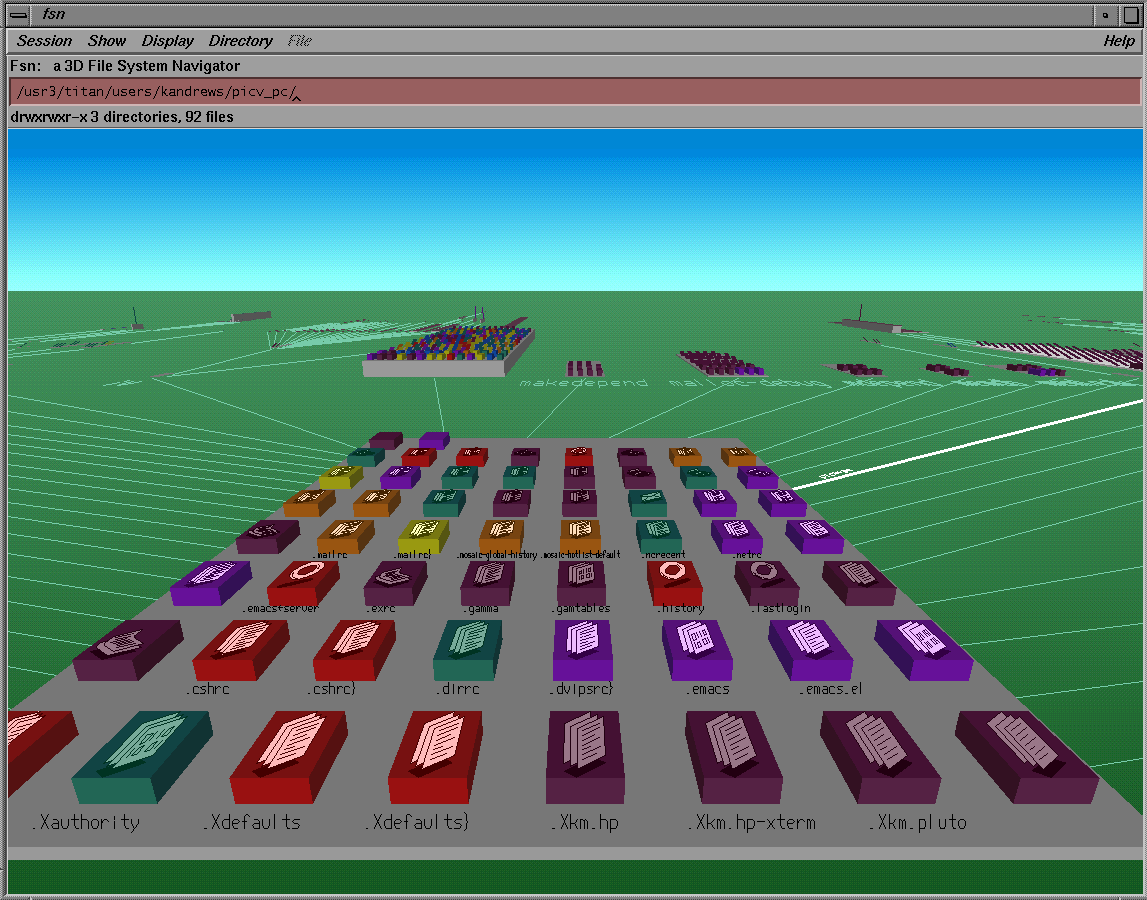
\includegraphics[width=8cm]{../grafik/fsn1.png}
\caption{FSN.}
\label{fig:fsn}
\end{figure}
\end{center}

\begin{center}
\begin{figure}[H]
    \centering
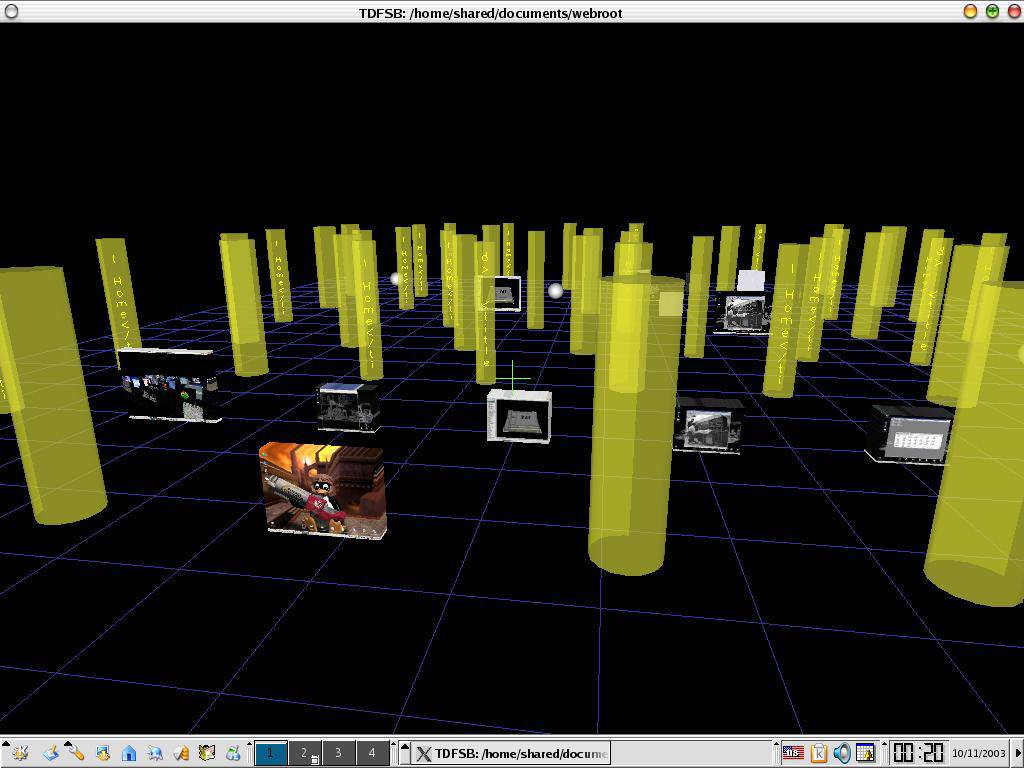
\includegraphics[width=8cm]{../grafik/tdfsb.jpg}
\caption{TDFSB.}
\label{fig:tdfsb}
\end{figure}
\end{center}

De ursprungliga obligatoriska kraven för produkten var följande:
\begin{LIPSkravlista}
\LIPSkrav{Original}{Alla filer ska representeras av block med någon textur på, är det en bild så ska bilden användas som textur}{1}

\LIPSkrav{Original}{Alla mappar ska representeras av block med någon textur}{1}
\LIPSkrav{Original}{Alla mappar och filer i en mapp ska vara placerade på en platta med en textur}{1}
\LIPSkrav{Original}{Ljussättningen ska ske med en Phong-shader}{1}
\LIPSkrav{Original}{Alla block ska ha skuggor}{1}
\LIPSkrav{Original}{Navigeringen ska vara first person där piltangenterna styr x och z koordinaterna och musen styr kameren i ett sfäriskt koordinatsystem}{1}
\LIPSkrav{Original}{Man ska inte kunna gå igenom filerna(collisions detection)}{1}
\LIPSkrav{Original}{Du ska kunna gå in i en mapp så transporteras du till den nya mappen)}{1}
\LIPSkrav{Original}{Du ska kunna klicka på en fil/mapp och få upp alla möjliga alternativ såsom radera, öppna...)}{1}
\LIPSkrav{Original}{Om du raderar en fil ska övriga filer ordna sig så det inte är några luckor någonstans}{1}
\LIPSkrav{Original}{Skydome ska finnas}{1}
\LIPSkrav{Original}{Endast Linux kommer stödjas}{1}
\end{LIPSkravlista}


och de ej obligatoriska kraven var följande:
\begin{LIPSkravlista}
\LIPSkrav{Original}{Du ska kunna få upp en terminal i filhanteraren}{2}
\LIPSkrav{Original}{Du ska kunna klicka på en mapp och sedan få upp en portal som du kan se in i mappen genom}{2}
\LIPSkrav{Original}{När du raderar en fil ska den explodera}{2}
\LIPSkrav{Original}{Innehåller en mapp många filer/mappar ska frustum culling användas för att minimera beräkningar}{2}
\LIPSkrav{Original}{Mapparnas texturer ska vara den ikon filen som operativsystemet använder med transparens, då ska renderingsordningen och vara korrekt}{2}
\end{LIPSkravlista}
Under projektets gång gick de obligatoriska kraven igenom en modifikation på grund av att projektet tog längre tid än vad jag trodde samt att en del inte riktigt passade in. Krav 5 togs bort på grund av tidsbrist, krav 6 gjordes om så att användaren bara navigerade i XZ planet då detta passade mycket bättre samt en del förenklingar kunde göras. Krav 9 togs bort då en terminal ansågs vara mycket enklare att implementera så all modifikation av filsystemet görs via den. Inga av de ej obligatorska kraven uppfylldes på grund av tidsbrist. I figur~\ref{fig:tmbtrf} kan man se resultatet. 
\begin{center}
\begin{figure}[H]
    \centering
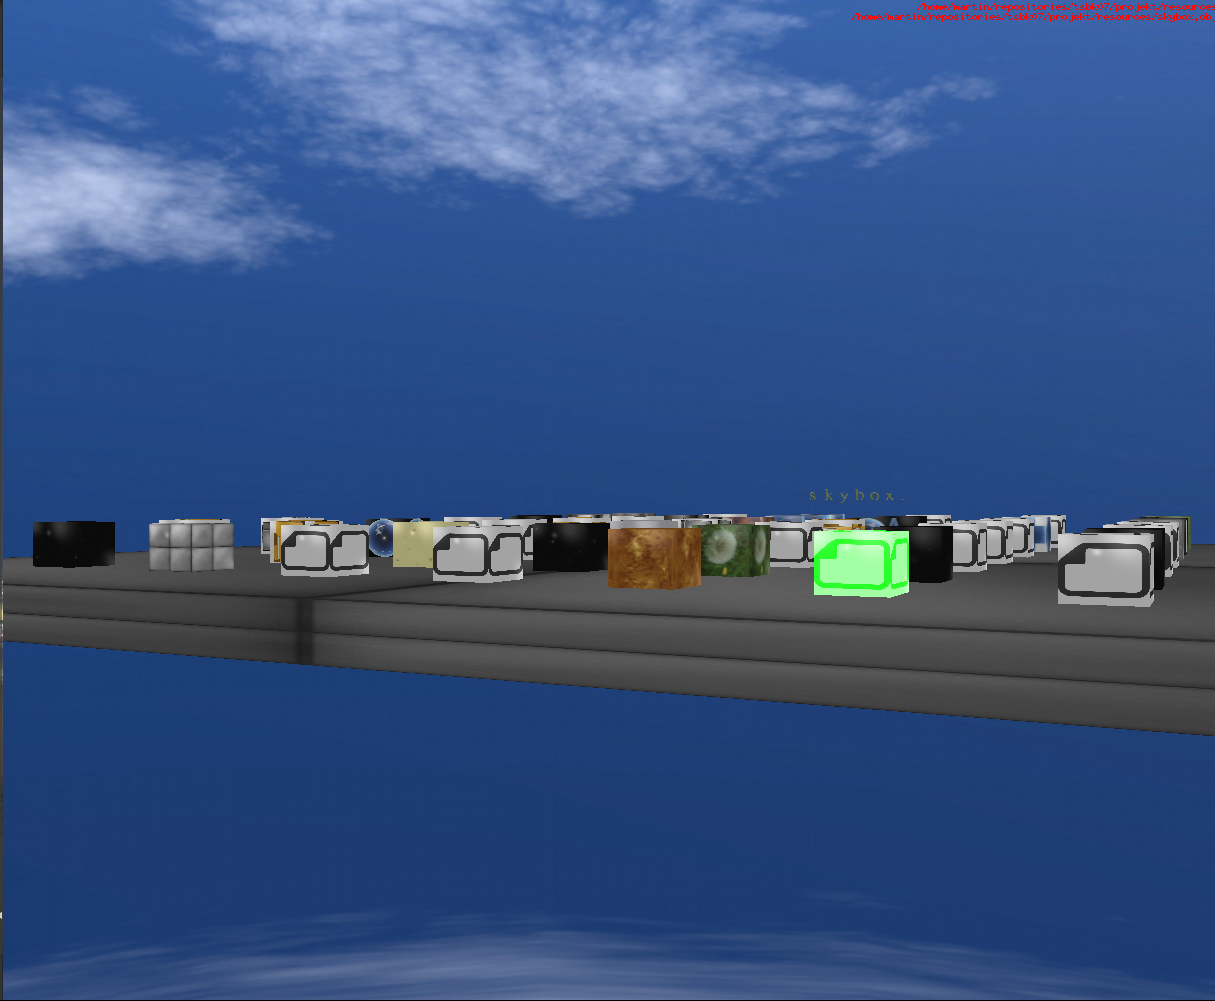
\includegraphics[width=8cm]{../grafik/tmbtrf.png}
\caption{TMBTRF.}
\label{fig:tmbtrf}
\end{figure}
\end{center}



\section{Bakgrund}
Det svåraste problemet jag hade innan jag började med projeketet var att på ett effektivt sätt interagera med datorns filsystem. Detta löstes rätt enkelt när jag upptäckte Boost::Filesystem. Detta bibliotek är inte speciellt använt så det finns inte så mycket hjälp att hitta på forum men dokumentation för det är väldigt bra så när jag väl kom in i det så fungera det väldigt bra. Funktioner såsom att byta namn och radera filer fanns redan implementerade så detta underlättade mycket.
\\
\\
Ett annat problem som var svårare än vad jag trodde var att visa filnamn i en 3D miljö. Den enklaste lösning skulle varit att använda något bibliotek för att generera texturer med en font till exempel FreeType. Jag försökte detta och jag kommer inte ihåg varför men jag fick det inte att fungera. För att få detta snyggt så skulle texturerna behöva vara transparenta så jag skulle behöva ta hänsynt till ordningen som alla objekt renderas. Min lösning på problemet var att generera .obj filer för alla tänkbara bokstäver och tecken som kan förekomma i ett filnamn. Jag valde alla bokstäver a-z och A-Z, alla siffror samt tecknen . - \_. Detta gjordes med ett python script i cad-programmet FreeCad. För att minimera inläsningstiden så läses alla dessa modeller in vid starten av programmet och återanvänds hela tiden. För att undvika problem som kan uppkomma vid långa filnamn som sträcker sig över hela miljön så visas bara de 7 första tecknen i filnamnet.
\\
\\
Anledningen till att C++ valdes var mest för dess datastrukturer såsom Vector, Map och string. Allting som kan göras i C++ kan självklart göras i C men där så är allting klart. Detta gjorde så att jag kunde göra en väldigt allmän klass som representerar alla objekt i 3D världen. Programmet arbetar också mycket med strängar och då är String väldigt mycket smidigare än en char array.
\\
\\
Ett problem som upptäcktes senare var att när man går in i en mapp som innehåller många filer, speciellt bilder, så tar det rätt lång tid innan hela världen har genererats. Detta skulle kunna lösas genom att ha en separat tråd som förbereder alla undermappar i den nuvarande mappen. Detta har dock inte implementeras men skulle jag fortsätta utveckla TMBTRF så skulle detta vara ett av de första problemen jag skulle lösa. 


\section{Implementation}
För att genomföra projektet så användes följande:
\begin{itemize}
\item C++ som programmeringsspråk fast en del bibliotek var skrivna i C
\item Objektorienterad kod
\item OpenGL för alla 3D effekter
\item X11 biblioteket för textöverläggning
\item OpenCV för inläsning av alla bilder och konvertering till ett format som OpenGl kunde använda
\item Boost::Filesystem för tillgång till datorns filsystem
\item MicroGlut för fönster och händelser hantering i OpenGL applikationen
\item VectorUtils3 för vektor och matrisoperationer
\item make för att snabbt kunna bygga hela programmet
\item Git för versionshantering
\item Eclipse som utvecklingsmiljö
\end{itemize}
\begin{center}
\begin{figure}[H]
    \centering
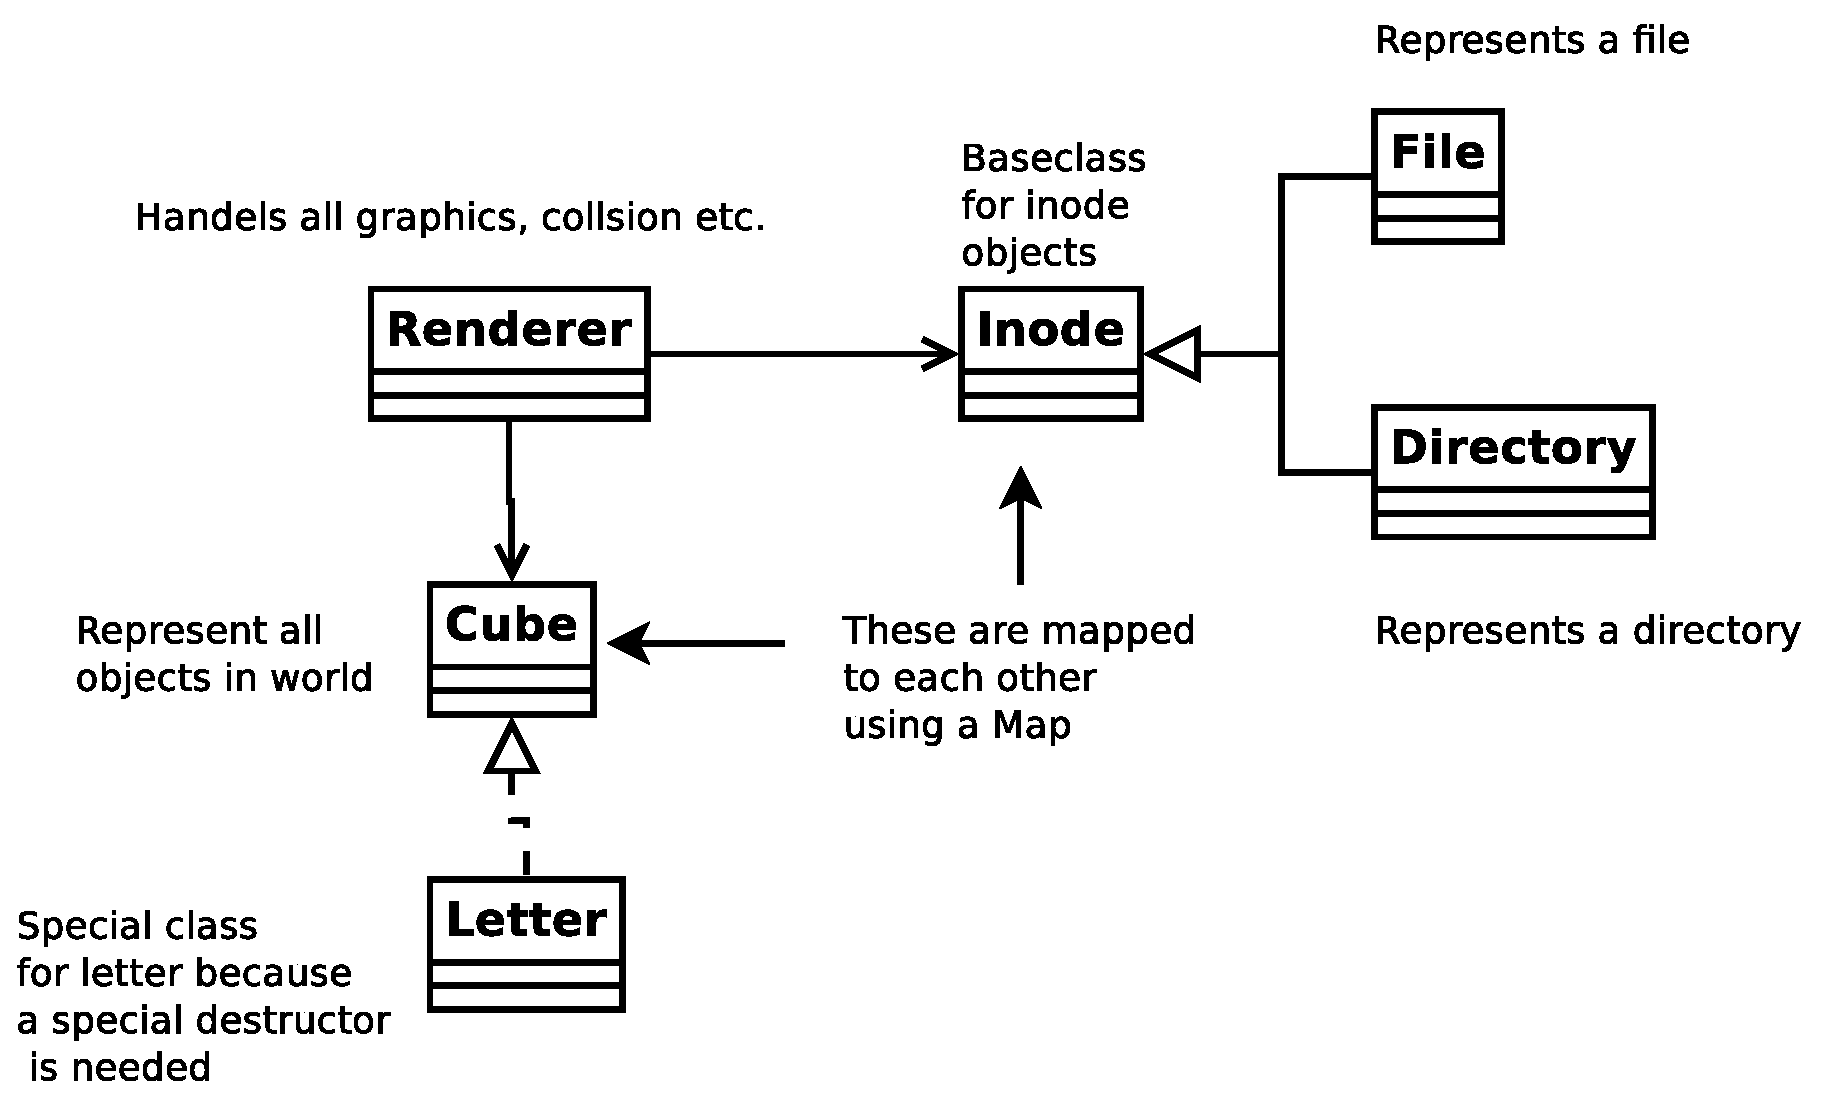
\includegraphics[width=10cm]{../grafik/uml.eps}
\caption{TMBTRF UML.}
\label{fig:uml}
\end{figure}
\end{center}
I figur~\ref{fig:uml} kan man se den grundläggande strukturen över programmet. Den är lite mer invecklad i verkligheten men den ger en bra överblick. När programmet startar så skapas först en Directory instans som representerar den mappen man startar programmet ifrån. Klassen Directory innehåller en Vector av Inodes objekt som representerar alla filer och mappar som ligger i den nuvarande mappen. Efter att denna vektor har initierats så skickas denna Directory instant in i en konstruktor för Renderer som skapar en Renderer instant med inititerar OpenGL applikationen med hjälp av MicroGlut. I konstruktorn så inititeras även en Vector i klassen som innehåller en massa Cube objekt som representerer golvet, skydomen och även alla filer och mappar. 
Om en Cube instans representerar ett Inode objekt så mappas dessa mot varandra med hjälp av en Map.
\\
\\
I början var även alla bokstäver ovanför alla Inodes objekt Cubes. Problemet med detta var att destruktorn för Cube raderar Model i klassen och eftersom alla bokstäver använder samma Model så blev alla bokstäver en Letter klass med en egen destruktorn som ej är virtuell så Cubes destruktor kallas ej på från Letters destruktor.
\\
\\
När alla Cube objekt har generetars så startar GLUTs loop och den kallar på Renderers display funktionen som i princip endast går igenom alla Cube objekt och kallar på varje objekts egna display funktion. Detta gör denna implementationen väldigt allmän och det är lätt att implementera nya objekt i världen. Till exempel så la jag till så jag kunde dra linjer i 3d världen vilket först endast var för att testa om pickingen fungerade som den skulle men sedan såg det rätt coolt ut så jag lät det vara kvar. Att implementera detta var väldigt lätt och krävde endast en ny funktion som genererade ett Cube objekt och en special display funktion för linjer. Renderers display funktion gör lite andra saker också såsom att kolla efter kollisioner och kolla om något objekt ska tas bort såsom linjer som endast existerar i 5 sekunder.

\subsection{Terminalen}
De kommandona som är implementerade är:
\begin{itemize}
\item select filename : som väljer en mapp/fil precis som om du skulle klicka på den 
\item help : som visar alla tillgängliga kommandon
\item cd directory : som gör att du går in i mappen precis som om du skulle gå in i den i världen
\item  rename filename new\_filename : som byter namn på filen
\item delete filename : som raderar filen
\end{itemize}
I cd, rename och delete kan du också skriva active istället för filnamnet så används den filen/mappen du har klickat på eller valt med select.

\subsection{Bygga programmet}
Skulle du vilja bygga programmet så måste det göras på en Linux dator med Microglut och Vectorutils3 i lib mappen för jag har modifierat båda med lite nya funktioner. Sedan behövs minst g++ version 4.9 för jag använder regex iterator som kom först i den versionen.

\section{Intressanta problem}
\subsection{Picking}
En av de sista sakerna jag implementerade var Picking så man kunde klicka på objekt i fönstret och välja filer och mappar. Jag trodde att detta skulle vara svårare men det var förvånansvärt lätt. Jag läste först om ett OpenGL hack där man renderar hela världen där varje objekt har olika färger och så kollar man vilken färg det är på pixeln som musen är på men detta verkade som ett rätt fult hack. Så istället så gjordes picking med hjälp av ray-casting. Jag fann väldigt mycket bra tips på denna hemsida \href{http://antongerdelan.net/opengl/raycasting.html}{Mouse Picking with Ray Casting}. 
\begin{center}
\begin{figure}[H]
    \centering
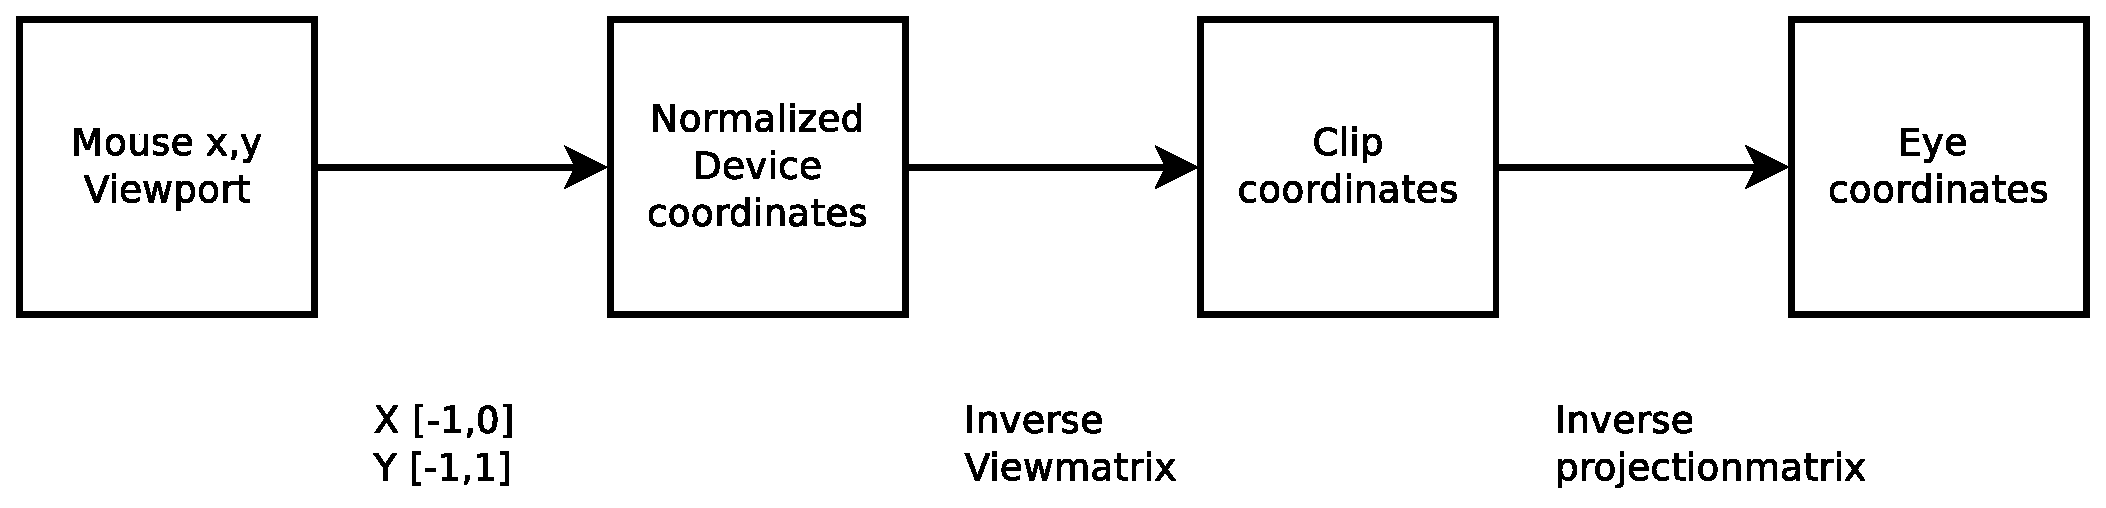
\includegraphics[width=8cm]{../grafik/picking.eps}
\caption{Picking.}
\label{fig:picking}
\end{figure}
\end{center}
Principen bakom picking med ray casting är helt enkelt att ta ett x och y värde på skärmen baklänges genom transformations pipelinen. 

\subsection{Texturer på alla bilder}
Alla filer som är bilder ska ha bilden som textur. Detta var lättare sagt än gjort. SOIL som är standarden vägrade fungera och CiMG gav bara svartvita bilder så till slut så valdes OpenCV för det är ett välbeprövat bibliotek som stödjer många filformat. De enda problemen med det var att OpenCV lagrar bilder från botten till toppen och OpenGL lagrar bilder från toppen till botten. Detta löstes genom att flippa bilden. Det andra problemet var ett OpenCV lagrar pixlar i BGR formatet men detta löstes med GL\_BGR som argument till glTexImage2D.

\subsection{Aliasing}
Något som syns väldigt tydligt i världen är aliasing då det är många kuber med skarpa kanter. Skulle jag fortsätta utveckla TMBTRF så skulle detta definitivt lösas med till exempel multisampling. 

\subsection{Text överläggning/regex}
Ett annat problem var att få upp en terminal ovanpå OpenGL. Detta löstes genom att använda X11 biblioteket och lägga på texten i fönstret efter att MicroGlut hade uppdaterat det. Detta gjorde att jag behövde få tillgång till fönsret och displayen samt skapa ett context för texten. Detta gjordes genom att modifiera MicroGlut. Jag ville också använda Regular expressions för att göra en så allmän terminal som möjligt men jag hade stora problem att få Regex att göra som jag ville. Den ansåg att fullständigt korrekta uttryck var fel så jag använde i slutändan rätt simpla uttryck kombinerat med tester om strängen från användaren innehöll en del ord för att välja rätt funktion.




\section{Sammanfattning}
Sammanfattningsvis så är jag nöjd med projektetet. Det har garanterat tagit mer tid än vad som normalt skulle krävas för ett projekt på två högskolepoäng men det har varit roligt att jobba på det. Jag skulle inte göra något annorlunda men det finns saker som jag skulle vilja ha gjort såsom anti-aliasing och förbereda undermapper och övermappen för att göra snabbare förflyttning mellan mappar. Det skulle vara snyggt om mappar blev portaler när du tryckte på dem så du kunde se in i den nya mappen. 
\\
\\
Överlag så har det varit ett lärorikt projekt och även hela kursen. Jag brukar inte gå på föreläsningar normalt men föreläsningarna i denna kurs har varit intressanta och roliga att gå på. Speciellt alla demonstrationer har varit givande.

\end{document}
